% ----------
% A LaTeX template for course project reports
%
% This template is modified from "Tech Report ala MIT AI Lab (1981)"
%
% ----------
\documentclass[12pt, letterpaper, twoside]{article}
\usepackage{geometry}
\usepackage[utf8]{inputenc}
\usepackage[english]{babel}
\usepackage[runin]{abstract}
\usepackage{titling}
\usepackage{booktabs}
\usepackage{fancyhdr}
\usepackage{helvet}
\usepackage{csquotes}
\usepackage{graphicx}
\usepackage{blindtext}
\usepackage{parskip}
\usepackage{etoolbox}

% preamble.tex
\geometry{letterpaper, top=2.2in, headheight=1.7in}
\date{}

\makeatletter

\def\fulltitle#1{\def\@fulltitle{#1}}
\def\runningtitle#1{\def\@runningtitle{#1}}
\def\runningauthor#1{\def\@runningauthor{#1}}
\def\affiliation#1{\def\@affiliation{#1}}
\def\department#1{\def\@department{#1}}
\def\memoid#1{\def\@memoid{#1}}
\def\theyear#1{\def\@theyear{#1}}
\def\mydate#1{\def\@mydate{#1}}

\runningtitle{Course Project Report}
\author{Student Name}
\runningauthor{Student Name}
\affiliation{Kennesaw State University}
\department{College of Computing and Software Engineering}
\memoid{CS 4632 Project}
\theyear{2026}
\mydate{June 11, 2026}

\def\displaymydate{\@mydate}
\def\displaytheyear{\@theyear}
\def\displaymemoid{\@memoid}
\def\displaydepartment{\@department}
\def\displayaffiliation{\@affiliation}
\def\displayrunningauthor{\@runningauthor}
\def\displayrunningtitle{\@runningtitle}

\makeatother

\makeatletter
\patchcmd{\@zfancyhead}{\fancy@reset}{\f@nch@reset}{}{}
\patchcmd{\@set@em@up}{\f@ncyolh}{\f@nch@olh}{}{}
\patchcmd{\@set@em@up}{\f@ncyolh}{\f@nch@olh}{}{}
\patchcmd{\@set@em@up}{\f@ncyorh}{\f@nch@orh}{}{}
\makeatother

\pagestyle{fancy}
\renewcommand{\headrulewidth}{0pt}

\fancypagestyle{firstpage}
{
    \fancyhf{}
    \fancyhead{%
        \begin{center}
            \textsc{\displayaffiliation}\\
            \textsc{\displaydepartment}
        \end{center}
        \vspace*{0.5in}
        \displaymemoid
        \hfill
        \displaymydate
    }
    \fancyfoot[L]{\footnotesize \textbf{\textsc{\displayaffiliation} -- \displaytheyear}}
}
\fancyhead[EL]{\small \displayrunningauthor}
\fancyhead[ER]{\small Page \thepage}
\fancyhead[OL]{\small Page \thepage}
\fancyhead[OR]{\small \displayrunningtitle}

\chead{}
\lfoot{}
\cfoot{}
\rfoot{}

\providecommand{\keywords}[1]{\noindent \textbf{Keywords:} #1}

\renewcommand{\familydefault}{\sfdefault}
\setlength{\parskip}{0.7em}
\setlength{\parindent}{0pt}
\abslabeldelim{:}
\setlength{\abstitleskip}{-\absparindent}

\pretitle{\Large \begin{center}}
\posttitle{\\[2ex] \Large \textbf{by}\end{center}}


% ----------
% Variables
% ----------

\title{\textbf{CS 4632 Course Project:\\
Discrete-Event Simulation of an Electronics Repair Department}}
\runningtitle{Electronics Repair Simulation}
\author{Carlos Guerrero}
\runningauthor{Carlos Guerrero}
\affiliation{Kennesaw State University}
\department{College of Computing and Software Engineering\\
CS 4632 -- Modeling and Simulation, Section W01}
\memoid{Milestone 1: Project Foundation}
\theyear{2026}
\mydate{June 11, 2026}

% ----------
% Actual document
% ----------

\begin{document}
\maketitle

\begin{abstract}
    \noindent
    This project will be a discrete-event simulation of the electronics repair support
    department where I work. The department repairs printed circuit boards and
    HVAC/refrigeration controllers. Jobs arrive from advance exchanges, production-line
    failures, reships, and customer Return Material Authorizations (RMAs). Customer RMAs
    wait on a physical rack, while the other work types are brought directly to the
    technicians. The model will represent two technicians, two
    test stations, priority rules, and interruptions for urgent production work. I will use
    historical data to compare turnaround time, RMAs, utilization,
    throughput, and repair outcomes.

\end{abstract}

\vspace{1cm}

\noindent
\textbf{Project repository:}\\
\texttt{https://github.com/CarlosG100/CS4632-Electronics-Repair}

\thispagestyle{firstpage}

\pagebreak

% ----------
% End of first page
% ----------

\newgeometry{}

\section{Project Overview}
\label{sec:overview}

\subsection{Domain and Problem}

The project is based on an electronics manufacturing support department. The department
receives PCBs and complete controller units, analyzes the failures, repairs what it can,
and records a final outcome. The workload is not constant because jobs/units arrive at
different times and repairs do not all take a uniform amount of time.

The main problem is deciding how priority rules and limited resources affect the different
job types. Urgent production failures need a fast response, but interrupting another repair
may increase the delay for normal customer work. A simulation is useful because the system
changes over time and includes random arrivals and repair times.

The project will answer these questions:

\begin{enumerate}
    \item How do first-in, first-out (FIFO) and priority with or without preemption affect turnaround time?
    \item How do technician specialization and station compatibility affect waiting and capacity?
    \item What practical change improves urgent response without creating a large RMA backlog?
\end{enumerate}

\subsection{Project Scope}

The model will begin when work reaches the department. It will include placement of customer
RMAs on the rack, direct handoff of other work, work selection, waiting, service,
interruption, completion, and outcome. It will also include the delayed return of a
defective advance-exchange unit.

The first model will represent general and specialized technician/station capabilities, but
it will not model individual technician efficiency, equipment downtime, parts delays, or
rework. About 80 percent of jobs can use either station, while about 20 percent require a
compatible technician and specialized station equipment. The model will use working hours rather than calendar hours, so nights
and weekends will not count toward repair time.
\section{System Description}
\label{sec:system}

\subsection{Entities, Events, State, and Resources}

The entities are the jobs or requests that flow through the department. Each one follows a
process based on its source. Customer RMAs are placed on a physical rack and selected in
FIFO order. Advance-exchange requests are brought to the department's attention by the RMA
administrator. Reships are brought by the receiving department, and production-line
failures are brought directly by production personnel. Job attributes include source,
priority, failure category, required capability, arrival time, service time, and final
outcome.

The main events are:

\begin{itemize}
    \item a customer RMA is placed on the rack or another work type is handed off;
    \item a technician begins or resumes work;
    \item an advance-exchange replacement is picked from stock, programmed, function
    tested, and handed to shipping;
    \item a repair is interrupted;
    \item a repair is completed;
    \item a job is repaired, scrapped, or returned to vendor (RTV); and
    \item a defective advance-exchange unit returns later as a customer RMA.
\end{itemize}

The state variables are the number of RMAs on the rack, direct requests waiting, work-in-process,
technician status, station status, resource capability, and the number of completed jobs.
The technicians and test stations are passive resources. The model includes two technicians
and two stations. Most work can use either technician/station pair, but specialized work
must wait for compatible resources.

\subsection{Work Selection and Service Process}

The proposed priority order is:

\begin{enumerate}
    \item advance exchange;
    \item urgent production-line failure;
    \item reship; and
    \item customer RMA.
\end{enumerate}

Customer RMAs remain on the rack until a technician is ready for another job, and the technician selects the oldest
RMA first. If that RMA requires specialized resources, it waits for the compatible
technician and station. Advance exchanges, reships, and production-line failures are direct
requests rather than jobs selected from the RMA rack. These direct requests will use the
priority order above when more than one needs attention. Only an urgent production failure
can interrupt work already in progress. The interrupted repair will keep its remaining
repair time and return to its prior waiting position. This allows the model to measure the
faster response for urgent work and the extra delay placed on normal work.

An advance-exchange request is preparation work rather than a repair. A technician will
pick a replacement unit from stock, take it to a compatible station, program it, and perform
a quick function test. The technician will then gather the required paperwork and return
the replacement to the shipping department. The station is only occupied during programming
and testing. When the defective field unit returns later, it will be created as a separate
normal-priority customer RMA repair job.

A reship is brought to the department by receiving. A technician will inspect the unit,
perform a function check at a compatible station, gather the new shipment paperwork,
and return it to shipping. Production-line personnel bring failed units directly to the
department for analysis and repair.

\subsection{Core Models and Concepts}

The project will use three main ideas:

\begin{enumerate}
    \item \textbf{Discrete-event simulation.} The simulation will use next-event time
    advance, meaning the clock jumps to the time of the next scheduled event, such as an
    arrival, repair start, interruption, or completion \cite{banks2005}.

    \item \textbf{FIFO work selection and priority rules.} Customer RMAs will be selected
    from the rack in FIFO order. Resource compatibility will be checked after selection.
    Direct requests will be represented separately, with production failures allowed to
    interrupt lower-priority work. This adapts Cobham's priority waiting-line concepts to
    the department's actual work-selection process \cite{cobham1954}.

    \item \textbf{Random input models.} Historical data will be used for arrival times,
    repair times, advance-exchange return delays, and repair outcomes \cite{law2015}.
\end{enumerate}

\subsection{Assumptions}

\begin{itemize}
    \item Approximately 80 percent of jobs can use either station and either technician.
    The remaining 20 percent require a compatible specialization.
    \item Customer RMAs are selected from the physical rack in FIFO order.
    \item Advance exchanges, reships, and production failures are brought directly to the
    technicians and are not selected from the RMA rack.
    \item Each active repair uses one technician and one compatible station. An
    advance-exchange request uses a technician throughout preparation, but it only uses a
    compatible station during programming and the quick function test.
    \item Interrupted repairs will continue from their remaining repair time.
    \item Replacement stock will be assumed available, and the selected replacement will
    pass its quick function test in the first version.
    \item The simulation clock and turnaround measurements will use department working hours.
    \item Parts inventory, rework, equipment downtime, and individual technician efficiency
    differences are outside the first version.
\end{itemize}

\section{Implementation Approach}
\label{sec:implementation}

\subsection{Language and Tools}

This will be a discrete-event simulation. I will write it in Python 3 using
SimPy because Python is readable and SimPy supports event timing, resources, and
interruptions. I will use Visual Studio Code for development. I will
write the job flow, FIFO rack-selection rules, direct-request priority logic, compatible
resource use, interruption logic, delayed RMA return, metrics, and experiments. 

\subsection{Historical Data}

The historical fields are job number, source, priority, arrival time,
repair start and end time, general failure category, required capability, outcome, and
advance-exchange request, preparation start, programming/test, shipping-handoff, and return
times.

For this model, repair service time means active working time between repair start and
completion. Time outside department working hours and known waits for parts will be removed.


\subsection{Outputs and Experiments}

Recorded measures will include RMAs, waiting direct requests, work-in-process,
turnaround time, waiting time, advance-exchange preparation time, resource use,
throughput, interruptions, and repair outcomes.

\begin{table}[ht]
\centering
\caption{Planned simulation scenarios}
\small
\begin{tabular}{p{0.35in} p{2.15in} p{2.4in}}
\toprule
\textbf{ID} & \textbf{Scenario} & \textbf{Purpose} \\
\midrule
0 & Two technicians and two compatible stations with preemption & Baseline system \\
1 & Priority without preemption & Measure the effect of interruption \\
2 & Handle all waiting work FIFO & Measure the effect of direct-request priority rules \\
3.1 & Add one technician & Test technician capacity and skill coverage \\
3.2 & Add one station & Test station capacity and equipment coverage \\
4 & Three technicians and three stations & Test a balanced capacity increase \\
5 & Higher arrival volume & Test a workload surge \\
6 & Add interruption overhead & Test the cost of preemption \\
\bottomrule
\end{tabular}
\end{table}

Each scenario will be run several times. I will compare average results and confidence
intervals instead of using only one simulation run.

\subsection{Eight-Week Timeline}

\begin{center}
\small
\begin{tabular}{p{0.4in} p{1.25in} p{3.75in}}
\toprule
\textbf{Week} & \textbf{Dates} & \textbf{Planned Work} \\
\midrule
1 & Jun. 3--7 & Select project and review initial course work. \\
2 & Jun. 8--14 & Complete M1: proposal, literature review, repository, and UML
diagrams. \\
3 & Jun. 15--21 & Prepare historical inputs and build the basic ob flow. \\
4 & Jun. 22--28 & Complete M2: initial implementation with priorities and
technician/station resources. \\
5 & Jun. 29--Jul. 5 & Add compatible resources, advance exchanges, reships,
and process details. \\
6 & Jul. 6--12 & Complete M3: full implementation with conditional waiting and
interruptions. \\
7 & Jul. 13--19 & Complete M4: run experiments, analyze outputs, and validate
the model. \\
8 & Jul. 20--23 & Complete M5: final report, results, repository, and video. \\
\bottomrule
\end{tabular}
\end{center}

\section{Literature Review}
\label{sec:literature}

\begin{itemize}
    \item Banks et al. explain discrete-event simulation through entities, queues, resources,
    events, and next-event time advance \cite{banks2005}. They also identify electronics
    assembly operations as a manufacturing use of simulation. This matches my project
    because controller and PCB jobs wait for limited resources, receive service, and leave
    with an outcome. I will adapt the basic service-system structure by adding an RMA rack,
    three direct-request sources, compatible technician/station resources, working hours,
    and interruptions.

    \item Law explains process-interaction simulation as following an entity through each step of a system \cite{law2015}. 
    This fits my project because each job moves through arrival, waiting, service, and completion. 
    I will also use Law's methods to create random inputs from historical data, run each scenario multiple times, 
    compare the results, and check event logs to verify that the simulation works correctly.

    \item Cobham shows that priority service reduces the waiting time of high-priority work
    at the cost of increasing the wait for lower-priority work \cite{cobham1954}. This is
    my main tradeoff: an urgent production failure may be handled faster
    while a normal customer RMA waits longer. I will adapt the priority model by using FIFO
    for the RMA rack, direct-request priorities, two compatible service resources, and both
    preemptive and non-preemptive scenarios. I will also test interruption overhead rather
    than assuming that stopping and restarting a repair has no cost.

    \item Little proves the relationship $L = \lambda W$ between average items in a system,
    throughput rate, and average time in the system \cite{little1961}. An important part of
    the result is that it does not depend on one specific arrival distribution, service
    distribution, number of channels, or queue discipline. I will use this relationship as
    a reasonableness check by comparing average work-in-process with throughput and average
    turnaround time from the simulation.

    \item Borshchev explains that service systems may require particular workers and shared
    equipment \cite{borshchev2020}. This supports modeling the 20 percent of jobs that need
    a specialized technician and station. He also warns that adding every real-world detail
    can make a model too large to manage. I will represent general and specialized
    capabilities while leaving individual efficiency, parts inventory, equipment downtime,
    and rework outside the first version.

\end{itemize}

\section{UML Diagrams}
\label{sec:uml}

Figure~\ref{fig:class-diagram} shows the main classes planned for the Python program.

\begin{figure}[ht]
\centering
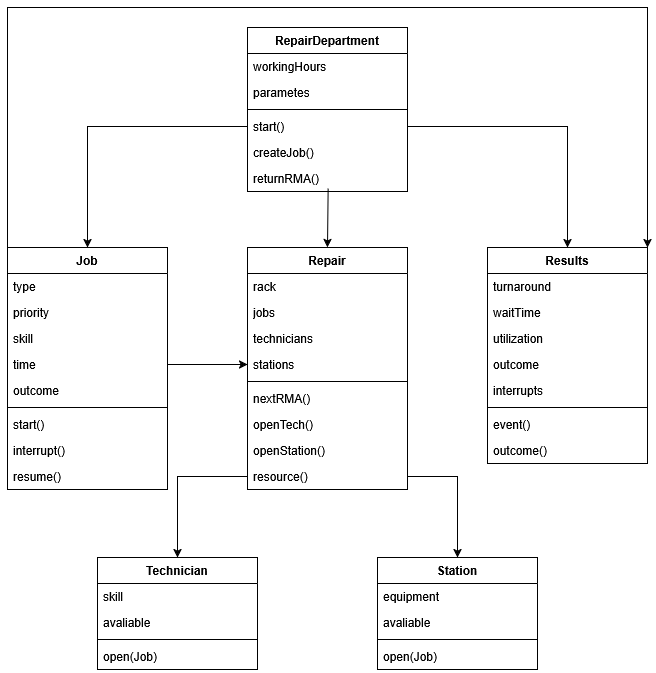
\includegraphics[width=0.78\textwidth]{class_diagram.png}
\caption{Basic class diagram for the simulation.}
\label{fig:class-diagram}
\end{figure}

\clearpage

\begin{figure}[p]
\centering
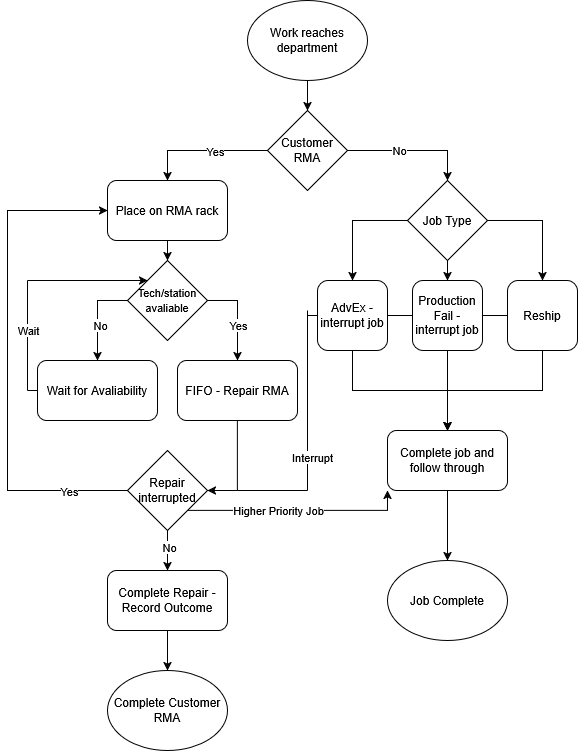
\includegraphics[height=7.2in]{activity_diagram.png}
\caption{Activity diagram for customer RMAs and directly delivered work.}
\label{fig:activity-diagram}
\end{figure}

\clearpage

\section{Verification, Validation, and Conclusion}
\label{sec:conclusion}

I will verify the model with small test cases, event traces, RMA rack-order checks, and checks
that technicians and stations are released correctly. The trace will follow state variables,
resource status, and job events after each important event. I will validate the model by comparing simulated arrivals, turnaround times,
throughput, and outcomes with the historical data.

The expected result is a model that shows whether the current priority process helps urgent
work without causing too much delay for customer RMAs. It should also show whether adding
a technician, a station, or a compatible resource combination would provide the most useful
improvement.

% ----------
% Bibliography
% ----------

\bibliography{references}
\bibliographystyle{abbrv}

\end{document}

% ----------
